\documentclass[14pt, a4paper]{article}
\usepackage[russian]{babel}
\usepackage{graphicx}
\usepackage{layout}
\usepackage[14pt]{extsizes}

\setcounter{tocdepth}{4}
\setcounter{secnumdepth}{4}

\usepackage{xcolor}
\usepackage{hyperref}

\usepackage{listings}
 % Цвета для гиперссылок
\definecolor{linkcolor}{HTML}{000000} % цвет ссылок
\definecolor{urlcolor}{HTML}{000000} %цвет гиперссылок

\hypersetup{pdfstartview=FitH,  linkcolor=linkcolor,urlcolor=urlcolor, colorlinks=true}

% \renewcommand{\section}{Глава}
% \usepackage{emoji}
% \setemojifont{Apple Color Emoji}

\definecolor{codegreen}{rgb}{0,0.6,0}
\definecolor{codegray}{rgb}{0.5,0.5,0.5}
\definecolor{codepurple}{rgb}{0.58,0,0.82}
\definecolor{backcolour}{rgb}{0.97,0.97,0.97}

\lstdefinestyle{mystyle}{
    backgroundcolor=\color{backcolour},   
    commentstyle=\color{codegreen},
    keywordstyle=\color{magenta},
    numberstyle=\tiny\color{codegray},
    stringstyle=\color{codepurple},
    basicstyle=\ttfamily\footnotesize,
    breakatwhitespace=false,         
    breaklines=true,                 
    captionpos=b,                    
    keepspaces=true,
    frame=single,                 
    % numbers=left,                    
    % numbersep=5pt,                  
    showspaces=false,                
    showstringspaces=false,
    showtabs=false,                  
    tabsize=2
}

\lstset{style=mystyle}

\oddsidemargin = 0pt
\marginparwidth = 45pt %57
\textwidth = 467pt
\textheight = 716pt
\topmargin = 0pt %17
\footskip = 30pt %30
\headheight = 0pt %12
\headsep = 0pt %25

% \setcounter{tocdepth}{1}

\begin{document}
\begin{titlepage}
    \topmargin=216pt
    \newpage
    \hangindent=0.7cm
    \huge ИУ-10\\
    Системное\\
    Программное\\
    Обеспечение\\
    Системы виртуализации\\
    \textbf{Вложенная
    виртуализация \\
    (nestedvirtualization)}

    \vspace{9cm}

    \begin{center}
        \small\textit{Москва, 2022}
    \end{center}
\end{titlepage}

\section*{На этом уроке}
\begin{enumerate}
    \item Изучим принципы реализации вложенных гипервизоров и её ограничения.
    \item Рассмотрим вариант построения окружения для исследования гипервизоров и экспериментов
    с ними.
\end{enumerate}

\tableofcontents \mbox{}\\

С повышением эффективности гипервизоров и увеличением быстродействия аппаратуры возникла и
была успешно реализована идея виртуализации гипервизора.\\

То есть внутри виртуальной машины запускается ещё один гипервизор, а поверх него запускаются
новые виртуальные машины. При всей странности такого подхода он находит всё большее
применение. Во-первых, он даёт возможность безопасно экспериментировать с самыми
разнообразными гипервизорами, не используя для этого дополнительную машину. Во-вторых, так
можно исследовать работу целых кластеров виртуальных машин. И в-третьих, можно использовать
традиционные преимущества виртуализации в рамках одного виртуального хоста, а это экономически
выгодно пользователям облачной инфраструктуры.
\newpage

\section*{Введение}
\addcontentsline{toc}{section}{Введение}

\begin{figure}[h]
    \centering
    \scalebox{1}{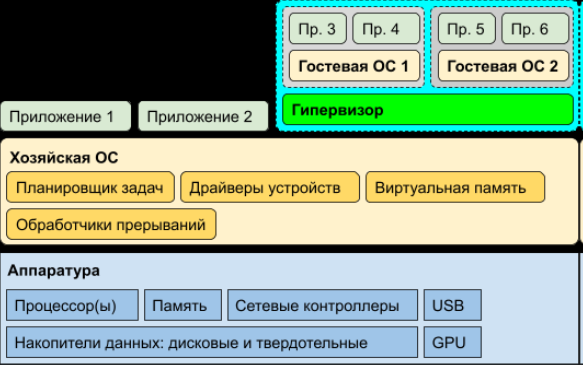
\includegraphics[width=1\textwidth]{1.png}}\\
    \small\textit{\href{https://tchubirabiron.wordpress.com/}{Ubuntu Inception}}
    \label{framework} 
\end{figure}

Читатель, который с нами прошёл исторический обзор систем виртуализации и освоил самые
распространённые гипервизоры, может задаться вопросом, зачем изобретать ещё один велосипед и
тратить время на реализацию очередного уровня абстракции. Именно так на первый взгляд
представляется вложенная виртуализация: мы будем запускать в первой гостевой системе ещё один
гипервизор, чтобы в его гостевой системе запустить что-то ещё.\\

Использование гипервизора первого уровня (не путать с гипервизором первого типа) уже позволяет
повысить эффективность использования аппаратуры и надёжность системы, изолировать разные
наборы программного обеспечения, всё ещё разделяя между ними одну и ту же аппаратуру и т.д.\\

Но надёжная изоляция гостевых систем друг от друга — это всего лишь убеждение. Мы видим всё
больше и больше атак на аппаратуру, которые позволяют получать доступ к данным не только
сторонних приложений и привилегированного ПО (читай: ядра операционной системы), но также и к
данным гипервизора, если он используется в данной системе, а заодно ещё и к данным других
гостевых систем. Так что стоит относиться к таким заявлениям с долей скепсиса.\\

Тут стоит остановиться на новой терминологии. В классических системах виртуализации гипервизор
существовал в единственном экземпляре на каждом компьютере или сервере, а потому гипервизор
был просто гипервизором. Однако мы собираемся запускать гипервизор как гостевую систему другого
гипервизора, получается матрёшка в матрёшке. Поэтому гипервизор, работающий максимально
близко к аппаратуре, мы будем называть гипервизором первого уровня, или хозяйским гипервизором.
Гипервизор, работающий поверх гипервизора первого уровня, мы будем называть гипервизором
второго уровня или гостевым гипервизором.\\

\begin{figure}[h]
    \centering
    \scalebox{1}{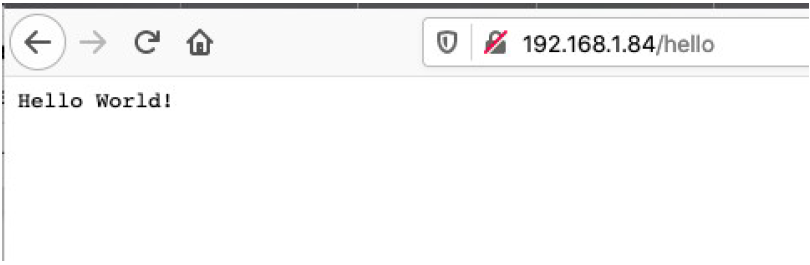
\includegraphics[width=1\textwidth]{2.png}}\\
    \label{framework} 
\end{figure}

\section*{Сферы применения вложенного гипервизора}
\addcontentsline{toc}{section}{Сферы применения вложенного гипервизора}

\subsection*{Исследование гипервизоров}
\addcontentsline{toc}{subsection}{Исследование гипервизоров}

Как мы узнали, изучая гипервизоры первого типа, некоторые из них весьма капризны к аппаратуре, на
которой их можно запустить. Лучший тому пример — VMware ESXi. Не имея доступа к весьма
ограниченному списку аппаратуры, запустить VMware ESXi на первом попавшемся компьютере или
сервере не удастся.\\

Однако гипервизор первого уровня может эмулировать устройства, которые удовлетворят
требованиям VMware ESXi. И действительно, VMware ESXi отлично работает как гостевая система
поверх Microsoft Hyper-V, KVM или Xen. Все три без проблем могут быть установлены на любой
64-битной x86-совместимой машине. Более того, таким образом можно проводить эксперименты с
гипервизором на какой-то рабочей системе. Например, на рабочий или домашний компьютер можно
запросто установить Oracle VirtualBox или VMware Workstation, а внутри установить любой другой
гипервизор. Теперь можно проводить любые эксперименты совершенно безопасно для основной
системы.\\

Стоит скептически относиться к вопросу полной безопасности экспериментов внутри виртуальных
машин. Гипервизоры, как и любое другое программное обеспечение, не лишены изъянов и проблем.
Поэтому некоторые действия гостевых систем могут приводить к краху не только самого гипервизора,
но и прочего ПО, работающего уровнями выше: гипервизора предыдущего уровня, операционной
системы, поверх которой запущен гипервизор и т. д. Так что стоит помнить о потенциальной
возможности краха системы и не использовать для опытов системы, выполняющие критически
важные задачи.

\subsection*{Исследование вычислительных кластеров}
\addcontentsline{toc}{subsection}{Исследование вычислительных кластеров}

Поверх гипервизора первого уровня можно запустить несколько виртуальных машин, в каждой из
которых установить ещё по гипервизору. У вас получится полноценный кластер, в котором возможно
экспериментировать с живой миграцией виртуальных машин, масштабированием, созданием
отказоустойчивых систем и т. д. Безусловно, производительность такого виртуального кластера будет
зависеть от количества ресурсов, которыми располагает реальная аппаратура тестового компьютера
или сервера. По производительности виртуальный кластер будет значительно уступать реальному
кластеру, состоящему из мощных серверов. То есть для решения «боевых» задач такая система будет
мало применима.\\

Тем не менее такая виртуальная лаборатория виртуализации даёт возможность познакомиться с
технологиями современной виртуализации в комфортных условиях и без значительных финансовых
затрат.

\subsection*{Повышение эффективности использования VDP/VPS}
\addcontentsline{toc}{subsection}{Повышение эффективности использования VDP/VPS}

Ещё один интересный сценарий использования вложенной виртуализации — повышение (да-да, ещё
большее повышение) эффективности хостинг-провайдеров. Если клиент уже арендовал
определённый набор ресурсов, почему бы эти ресурсы не разделить на решение нескольких задач?
Например, на одном арендованном VPS/VDS можно запустить одновременно почтовый сервер, базу
данных и веб-сервер, но не просто как разные процессы в одной ОС, а скорее как контейнеры,
изолированные друг от друга виртуальными машинами.\\

Возможно, такой сценарий выглядит несколько необычно, но такого рода хостинг экономически
выгоден, поэтому спрос на него вскоре должен повыситься. Более того, мы уже наблюдаем
возможность использования вложенной виртуализации на основной инфраструктуре крупных
хостингов, таких как Digital Ocean, \href{https://cloud.google.com/compute/docs/instances/nested-virtualization/overview}{Google Cloud},\href{https://community.oracle.com/hub/blogs/gmelo/2017/10/04/kvm-nested-virtualization-on-oracle-cloud-infrastructure}{Oracle Cloud}.

\subsection*{Обеспечение повышенной безопасности внутри
виртуальной машины}
\addcontentsline{toc}{subsection}{Обеспечение повышенной безопасности внутри виртуальной машины}

Одно из преимуществ запуска ПО внутри виртуальной машины — высокая изоляция этого ПО, то есть
существенное затруднение злонамеренных действий по отношению к другому ПО, запущенному на
этой аппаратуре. И если виртуальные машины достаточно давно стали использоваться в
операционных системах для запуска подозрительного ПО, то как быть в случае, если сама ОС
запущена в виртуальной машине? Тут-то и приходит на выручку вложенная виртуализация.\\

В конце 2018 года компания Microsoft рассказала об очень интересном нововведении в будущих
версиях операционной системы Windows 10, начиная со сборки 1903, — Windows Sandbox, или 
«песочница Windows» в переводе на русский. Windows Sandbox позволяет незаметно для
пользователя запускать отдельные приложения в окружении виртуальной машины Microsoft Hyper-V,
используя текущее состояние основной системы как точку старта. Больше об этом можно прочитать в
\href{https://remontka.pro/sandbox-windows-10/}{статье «Песочница Windows 10 — как включить, настроить и использовать».}

\section*{Реализация гипервизора поверх гипервизора}
\addcontentsline{toc}{section}{Реализация гипервизора поверх гипервизора}

\subsection*{Программная эмуляция в хозяйском гипервизоре}
\addcontentsline{toc}{subsection}{Программная эмуляция в хозяйском гипервизоре}

Как мы помним, сама по себе виртуализация — это не фундаментально сложная задача. В конце
концов, можно программно эмулировать оборудование любой сложности с любой степенью точности.\\

Самый простой пример — запуск вложенных виртуальных машин, не требующих аппаратной
поддержки виртуализации. На x86-платформе — это запуск 32-битных гостевых систем. То есть в
Oracle VirtualBox или VMware Workstation можно установить 32-битную систему, причём неважно,
будет это Linux-дистрибутив или Windows. Внутри этой системы установить ещё один экземпляр
Oracle VirtualBox или VMware Workstation и в нём установить ещё одну полноценную систему.\\

Вопрос лишь в том, какую цену мы готовы за это заплатить. Как и в случае обыкновенной (не
вложенной) виртуализации, самый интересный вопрос: как реализовать вложенную виртуализацию
максимально эффективно, то есть таким образом, чтобы гостевые системы самого высокого уровня
исполнялись со скоростью, максимально близкой к запуску непосредственно на аппаратуре.\\

Так как аппаратура с 64-битными процессорами становится всё более распространённой, всё
сложнее найти 32-битное ПО. В частности, популярный Linux-дистрибутив Ubuntu прекратили
выпускать в версии для 32-битных систем, начиная с релиза 17.10 Artful Aardvark, а потому
используйте более ранние версии, например 16.04 LTS.

\subsection*{Аппаратная виртуализация в хозяйском гипервизоре}
\addcontentsline{toc}{subsection}{Аппаратная виртуализация в хозяйском гипервизоре}

Тут самое время вспомнить, как достигается высокая эффективность классической виртуализации —
за счёт выполнения максимального объёма работы непосредственно гостевой системой. Именно для
этого были реализованы дополнительные аппаратные расширения, позволяющие запускать гостевые
системы так, как если бы они работали непосредственно на аппаратуре. Лишь в относительно редких
ситуациях они «вываливаются» в режим гипервизора для обработки особенных случаев. И именно
частота возникновения таких особенных случаев, обработку которых мы не готовы доверить гостевой
системе, определяет эффективность системы виртуализации в целом.\\

То есть для эффективной виртуализации второго уровня необходимо сделать так, чтобы большая
часть работы выполнялась непосредственно в гостевой системе. Возможности современной аппаратуры, 
в первую очередь центральных процессоров, а также некоторых периферийных
устройств позволяют осуществить это. Нужно лишь, чтобы гостевой гипервизор использовал такие же
средства аппаратного ускорения виртуализации, которые доступны хозяйскому гипервизору. И, как ни
странно, компания AMD позаботилась об этом с самого начала: команды управления виртуализацией
также могут быть виртуализованы, то есть могут корректно выполняться гостевой системой.\\

Благодаря такой аппаратной поддержке вложенная виртуализация была реализована для
процессоров AMD почти на годы раньше, чем для процессоров Intel. Потому как в случае Intel мы
сталкиваемся со вполне ожидаемым ограничением: даже самые современные процессоры Intel не
имеют аппаратной поддержки вложенной виртуализации. То есть фактически только хозяйский
гипервизор может полноценно управлять всем оборудованием и обрабатывать исключительные
состояния, генерируемые его гостевыми системами, то есть и гостевыми гипервизорами, и их гостями.
Чтобы гостевые гипервизоры могли создавать эффективные виртуальные машины, гипервизору
потребовалось бы иметь возможность, выполняя команды VMX, настраивать окружение для запуска
гостевых систем и в дальнейшем управлять гостями. Но это по определению невозможно.\\

Решение этой, казалось бы, неразрешимой проблемы состоит в старой доброй эмуляции. Но
эмулировать нужно только VMX-команды, выполняемые гостевым гипервизором. Мы помним, что всё
равно в один момент времени процессором выполняется только одна последовательность команд,
будь то хозяйский гипервизор или гость гостевого гипервизора. Можно реализовать многоуровневую
виртуализацию путём мультиплексирования нескольких уровней виртуализации в один уровень,
реализованный аппаратурой. Другими словами, и гостевой гипервизор, и его гости выполняются в
одном и том же режиме процессора, однако обработка исключительных ситуаций, сгенерированных
гостевой системой любого уровня, начинается всегда хозяйским гипервизором. При необходимости её
может продолжить гостевой гипервизор, если эта исключительная ситуация была вызвана его
гостевой системой.\\

\begin{figure}[h]
    \centering
    \scalebox{0.75}{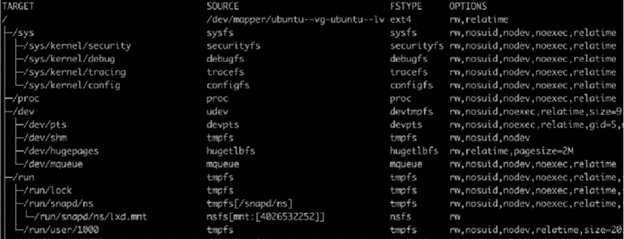
\includegraphics[width=1\textwidth]{3.png}}\\
    \small\textit{Обработка исключительной ситуации процессором без аппаратной поддержки вложенной виртуализации}
    \label{framework} 
\end{figure}

То есть в реальности система, реализующая вложенную виртуализацию на современных процессорах
Intel и AMD, выглядит не так:

\newpage

\begin{figure}[h]
    \scalebox{0.75}{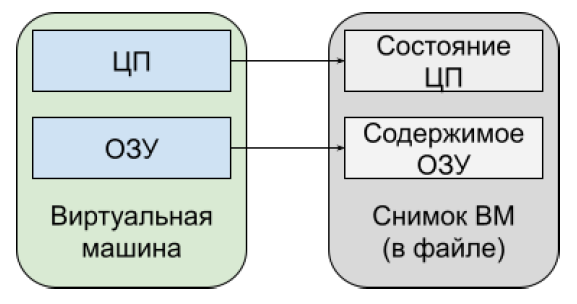
\includegraphics[width=1\textwidth]{4.png}}
    \label{framework} 
\end{figure}

\begin{figure}[h]
    А вот так:\\

    \scalebox{0.75}{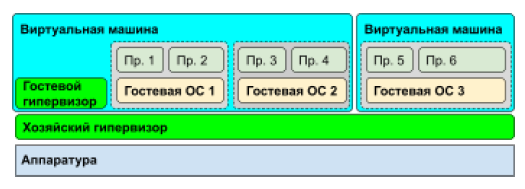
\includegraphics[width=1\textwidth]{5.png}}
    \label{framework} 
\end{figure}

Такая реализация вложенной виртуализации хороша как минимум по двум причинам:
\begin{enumerate}
    \item Она возможна на любых процессорах Intel с уже имеющейся аппаратной поддержкой
    виртуализации, то есть нет ограничения на использование только какого-то нового поколения
    процессоров. Другими словами, она, будучи сугубо программной реализацией, позволяет
    использовать вложенную виртуализацию на огромном парке уже существующего
    оборудования.
    \item Позволяет реализовать вложенную виртуализацию любого порядка. То есть в теории может
    быть хоть пять, хоть десять уровней виртуализации.
\end{enumerate}

Однако стоит помнить, что эмуляция, особенно многоуровневая, как в случае вложенной
виртуализации, когда эмулируемая команда гостевой системы самого высокого уровня
обрабатывается последовательно гипервизорами всех уровней, становится весьма затратной.
Эффективность системы в целом стремительно снижается с добавлением каждого нового уровня
виртуализации.

\subsection*{Оценка производительности вложенного гипервизора}
\addcontentsline{toc}{subsection}{Оценка производительности вложенного гипервизора}

Интересно посмотреть на реальных примерах, в каких случаях и как сильно различается
производительность систем при запуске в хозяйском и гостевом (вложенном) гипервизоре. Ещё
интереснее понять, вложенность какого порядка ещё имеет смысл использовать, а когда уже
пропадает практическая ценность дополнительной вложенности.\\

\href{https://www.usenix.org/}{Первоначальные оценки} показали, что накладные расходы на обслуживание первого гостевого
гипервизора всего на 6–8\% выше, чем при работе одного только хозяйского гипервизора.\\

На более свежем оборудовании (\href{https://www.intel.com/content/www/us/en/support/ru-banner-inside.html}{Intel VMCS shadowing}, 
\href{https://www.intel.com/content/www/us/en/support/ru-banner-inside.html}{Intel vAPIC или APICv}) и с более
совершенным ПО производительность гостевого гипервизора первого порядка при нагрузках
некоторых типов едва ли отличима от хозяйского гипервизора. Разумеется, оценивается
производительность не самого гипервизора, а его гостевой системы. Подробности можно прочитать в
статьях \href{https://www.redhat.com/en/blog/inception-how-usable-are-nested-kvm-guests}{Inception: How usable are nested KVM guests} 
и \href{https://blogs.technet.microsoft.com/larryexchange/2015/12/29/performance-overhead-of-nested-virtualization-on-windows-server-2016-technical-preview-4/}{Performance Overhead of Nested Virtualization on Windows Server 2016 Technical Preview 4.}

\section*{Примеры реализации}
\addcontentsline{toc}{section}{Примеры реализации}

Когда мы уже ознакомились с теоретической частью, интересно узнать, как можно получить опыт
работы с вложенными гипервизорами. К счастью, на сегодняшний день самые используемые
гипервизоры для x86-платформы имеют полноценную поддержку вложенной виртуализации. Мы же
рассмотрим только два варианта (KVM и Hyper-V). Эксперименты с ними более доступны и в смысле
выбора подходящей аппаратуры, и в смысле установки и настройки гипервизора. При желании можно
с лёгкостью найти инструкции и для других гипервизоров:

\begin{itemize}
    \item \href{https://wiki.xenproject.org/wiki/Nested_Virtualization_in_Xen}{Nested Virtualization in Xen};
    \item \href{https://www.virtuallyghetto.com/2012/08/how-to-enable-nested-esxi-other.html}{How to Enable Nested ESXi \& Other Hypervisors in vSphere 5.1};
    \item \href{https://www.altaro.com/vmware/deploying-nested-esxi-is-easier-than-ever-before/}{Deploying nested ESXi is easier than ever before}.
\end{itemize}

\newpage
\subsection*{KVM как хозяйский гипервизор}
\addcontentsline{toc}{subsection}{KVM как хозяйский гипервизор}

\begin{figure}[h]
    \centering
    \scalebox{1}{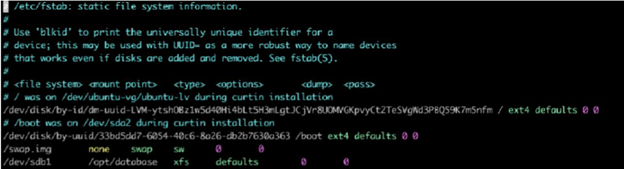
\includegraphics[width=1\textwidth]{6.png}}\\
    \small\textit{Ubuntu 18.04.3 c гостевой системой Ubuntu 18.04.3 в роли гостевого гипервизора с ещё одной гостевой системой с
    Ubuntu 18.04.3}
    \label{framework} 
\end{figure}

Начнём рассматривать примеры реализации вложенной виртуализации с набирающего популярность
гипервизора KVM. Из обзора гипервизоров первого типа на предыдущем занятии мы знаем, что KVM
можно запросто установить на компьютер или сервер с современным 64-битным процессором Intel
или AMD, имеющим поддержку аппаратной виртуализации (Intel VT-x и AMD SVM, соответственно), с
установленным более-менее современным Linux-дистрибутивом. Более того, все части программного
обеспечения свободно доступны, так как это ПО с открытым исходным кодом.

\subsubsection*{Установка и конфигурация}
\addcontentsline{toc}{subsubsection}{Установка и конфигурация}

Будем исходить из того, что гипервизор KVM уже установлен в системе и мы проверили возможность
создавать обыкновенные виртуальные машины. Затем следует проверить, доступна ли поддержка
вложенной виртуализации на данной конкретной системе. Если вложенная виртуализация возможна,
нужно включить её поддержку в соответствующем модуле ядра Linux.\\

Есть простая и понятная \href{https://docs.fedoraproject.org/en-US/quick-docs/using-nested-virtualization-in-kvm/}{инструкция на английском языке} 
и примерно \href{https://bogachev.biz/2019/05/27/vklyuchenie-nested-virtualizacii-v-kvm/}{то же самое на русском}.\\

Вся настройка сводится к двум шагам, а при использовании хозяйской системы с ядром Linux версии
старше 4.20 или с процессорами AMD — всего к одному. Например, в случае Ubuntu это относится
именно к третьему обновлению — 18.04.3. Предыдущие, 18.04 и 18.04.2, использовали ядра,
соответственно, 4.15 и 4.18. Можно также начинать с версии 19.04. В случае Fedora — с версии 30.

\begin{enumerate}
    \item Включить поддержку вложенной виртуализации в соответствующем модуле ядра:
    \begin{enumerate}
        \item[a.] Для процессоров AMD она по умолчанию включена уже почти десять лет. Можно разве
        что проверить, действительно ли включена поддержка:
        \begin{lstlisting}
# cat /sys/module/kvm_amd/parameters/nested
Y
        \end{lstlisting}
        \item[b.] Для процессоров ядра Linux версии ниже 4.20 необходимо явно включить поддержку
        вложенной виртуализации при загрузке соответствующего модуля, предварительно его
        выгрузив:
        \begin{lstlisting}
# modprobe -r kvm_intel
# modprobe kvm_intel nested=1
# cat /sys/module/kvm_intel/parameters/nested
Y
        \end{lstlisting}   
    \end{enumerate}

    \item Дать указание хозяйскому гипервизору предоставлять виртуализированные ресурсы
    управления виртуализацией своим гостям. Для этого нужно установить модель эмулируемого
    процессора в значение \\
    \colorbox{backcolour}{host-passthrough}.\\
    Это проще всего сделать в графическом интерфейсе диспетчера виртуальных машин, в меню
    настройки процессора, поле Model:
    \begin{figure}[h]
        \begin{centering}
        \scalebox{0.85}{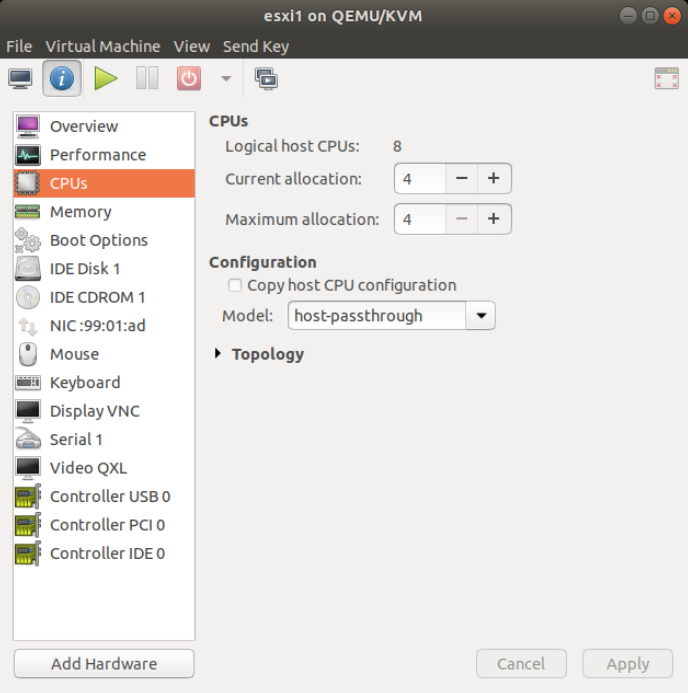
\includegraphics[width=1\textwidth]{7.png}}\\  \mbox{}\\
        \label{framework} 
        \end{centering}
        В результате после установки ОС в гостевой системе мы обнаруживаем, что и там есть аппаратная
поддержка виртуализации, да ещё и вложенной:
    \end{figure}
    
    \begin{lstlisting}
# sudo virt-host-validate
  QEMU: Checking for hardware virtualization                  : PASS
  QEMU: Checking if device /dev/kvm exists                    : PASS
  QEMU: Checking if device /dev/kvm is accessible             : PASS
  QEMU: Checking if device /dev/vhost-net exists              : PASS
  QEMU: Checking if device /dev/net/tun exists                : PASS
...

# cat /sys/module/kvm_intel/parameters/nested
Y
    \end{lstlisting}
\end{enumerate}

\subsubsection*{Особенности}
\addcontentsline{toc}{subsubsection}{Особенности}

Как мы уже упоминали выше, поддержка вложенной виртуализации зачастую включена по
умолчанию. Интересно, что ввиду более продуманной аппаратной реализации SVM в процессорах
AMD программная реализация вложенной виртуализации для процессоров AMD была полноценно
реализована почти на 10 лет раньше, чем для процессоров Intel.\\

Поддержка вложенной виртуализации включена по умолчанию:
\begin{itemize}
    \item для процессоров AMD с поддержкой SVM в версии ядра Linux 2.6.32, выпущенного в начале
    декабря 2009 года;
    \item \href{https://git.kernel.org/pub/scm/linux/kernel/git/torvalds/linux.git/commit/?id=1e58e5e59148916fa43444a406335a990783fb78}{для процессоров Intel с поддержкой VT-x в версии ядра Linux 4.20}, которое было выпущено в
    конце декабря 2018 года.
\end{itemize}

Сейчас крупнейшие провайдеры облачных сервисов, такие как Google и Oracle, активно используют
вложенную виртуализацию с хозяйским гипервизором KVM и продолжают совершенствовать
программную реализацию самого гипервизора.\\

Ещё стоит отметить универсальность KVM как гостевого гипервизора, так как в гостевой системе
возможно легко установить любой другой гипервизор для архитектуры x86: Xen, Microsoft Hyper-V,
VMware ESXi и т. д.\\

\newpage

\subsection*{Microsoft Hyper-V как хозяйский гипервизор}
\addcontentsline{toc}{subsection}{Microsoft Hyper-V как хозяйский гипервизор}

\begin{figure}[h]
    \centering
    \scalebox{1}{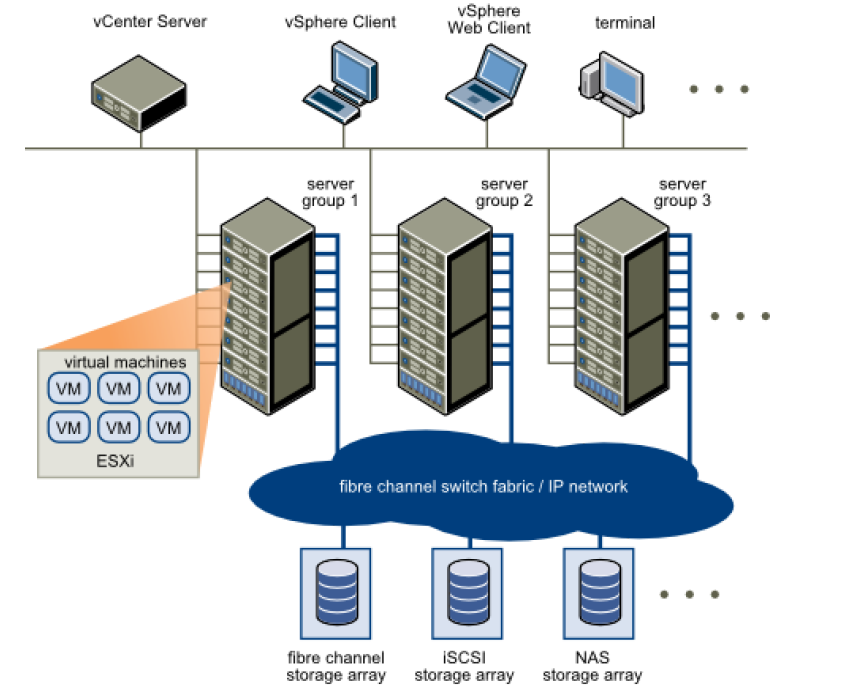
\includegraphics[width=1\textwidth]{8.png}}\\  \mbox{}\\
    \label{framework} 
\end{figure}

Так как Microsoft Hyper-V — это современный высокопроизводительный гипервизор, разумеется, он
поддерживает вложенную виртуализацию. Лабораторию по исследованию виртуализации возможно
организовать на любой машине с Windows 10, начиная с Anniversary Update, то есть с версии 1607 и
более свежих.

\newpage

\subsubsection*{Установка и конфигурация}
\addcontentsline{toc}{subsubsection}{Установка и конфигурация}

В отличие от KVM, в случае с Hyper-V поддержку вложенной виртуализации необходимо в явном виде
включать для каждой конкретной виртуальной машины. Причём делается это исключительно из
консоли PowerShell от имени администратора следующей командой:

\begin{lstlisting}
Set-VMProcessor -VMName <VMName> -ExposeVirtualizationExtensions $true
\end{lstlisting}

Рекомендуем ознакомиться с \href{https://learn.microsoft.com/en-us/virtualization/hyper-v-on-windows/user-guide/nested-virtualization}{официальной статьей Microsoft о вложенной виртуализации}.

\subsubsection*{Особенности}
\addcontentsline{toc}{subsubsection}{Особенности}

Как обозначено в приведённой выше статье, сейчас вложенная виртуализация поддерживается
только для процессоров Intel. Это, с одной стороны, выглядит несколько странно, ведь в процессорах
AMD более удачная аппаратная реализация расширений для ускорения виртуализации. С другой
стороны, до последнего времени на рынке серверной аппаратуры доминировали процессоры
производства Intel, а потому им, очевидно, уделяли больше внимания.\\

Тем не менее стремительно набирают популярность процессоры AMD семейства Ryzen, неожиданно
тесня Intel, \href{https://www.extremetech.com/computing/299191-amds-server-market-share-could-more-than-double-by-the-end-of-2020}{в том числе и на рынке серверов}. Так что можно предположить, что компания Microsoft в
ближайшее время реализует поддержку вложенной виртуализации и для процессоров производства
AMD.\\

\href{https://ru.wikipedia.org/wiki/Ryzen}{Ryzen} — торговая марка 64-битных x86-совместимых микропроцессоров, разрабатываемых и
продаваемых компанией AMD для настольных, мобильных и встроенных систем, основанных на
микроархитектурах Zen, Zen+ и Zen 2.

\section*{Заключение}
\addcontentsline{toc}{section}{Заключение}

На конец 2019 года осталась единственная не до конца решённая проблема с вложенной
виртуализацией — это миграция гостевых гипервизоров. Над решением этой проблемы работают
инженеры таких компаний, как Red Hat, Microsoft, Oracle и т. д.\\

Благодаря зрелости и аппаратуры, и ПО, использующего аппаратные расширения для ускорения
виртуализации, мы наблюдаем значительно возросшее быстродействие вложенной виртуализации и
её стабильность. Можно предположить, что скоро вложенную виртуализацию начнут использовать всё
более широко даже в «боевых» условиях. Ранее вложенная виртуализация находила применение
только в лабораториях или любительских решениях. Как мы упоминали в начале урока, Google Cloud
и Oracle Cloud используют вложенную виртуализацию в своих продуктах. Более того, в случае с Oracle
вложенная виртуализация — это \href{https://blogs.oracle.com/}{ключевая особенность их инфраструктуры}.\\

\section*{Виртуализация устройств ввода-вывода}
\addcontentsline{toc}{section}{Виртуализация устройств ввода-вывода}

Единственная способность компьютера — обработка данных. Будь то реальная или виртуальная
машина, ей требуется обеспечить доступ к данным для обработки. Мы рассмотрим механизмы
взаимодействия с аппаратурой ввода-вывода, используемые в современных гипервизорах.\\

Изначально концепция виртуализации подразумевала создание полноценной копии исходного
оборудования и предоставление экземпляра такой копии пользователю, чтобы ему казалось, что в его
пользование предоставлена реальная машина. Такой подход до сих пор широко распространён, но он
приводит к заметному снижению эффективности системы виртуализации из-за необходимости
эмулировать реальную аппаратуру. Как мы помним, в современных центральных процессорах есть
специальные режимы работы для реализации эффективной виртуализации. Они позволяют вместо
эмуляции выполнять бинарный код непосредственно реальным процессором. Таким образом
производительность вычислений в виртуальной машине максимально приближена к
производительности той же системы без использования виртуализации.\\

Но сами по себе вычисления не представляют интереса, если нет данных, над которыми
производятся те самые вычисления. А данные поступают от внешних устройств, которые их хранят
или связывают процессор с внешним миром. Думаем, понятно, что скорость, с которой
осуществляется доступ к данным, сильно сказывается на общей производительности системы. А
потому эффективная работа устройств ввода-вывода данных — немаловажный аспект в деле
повышения эффективности системы виртуализации.\\

Эмуляция реального оборудования — пожалуй, не лучшее решение. Более эффективные и
популярные варианты: паравиртуализация, проброс оборудования непосредственно в гостевые
системы, а также драйверы в пространстве пользователя. Обо все этих вариантах мы поговорим
ниже.

\section*{Паравиртуализация оборудования}
\addcontentsline{toc}{section}{Паравиртуализация оборудования}

Идея паравиртуализации состоит в том, чтобы вместо трудоёмкой и неэффективной эмуляции
реального оборудования со всеми важными деталями, такими как регистры управления, буферы
обмена данными, прерывания, эмулировать виртуальное устройство.\\

Такой способ повышения эффективности систем ввода-вывода виртуальных машин появился
первым, и к настоящему моменту все гипервизоры в той или иной степени поддерживают некоторый
набор паравиртуализованных устройств. Несмотря на то, что разработчики различных гипервизоров
изначально предлагали свои собственные паравиртуализованные устройства, сегодня VirtIO стал
стандартом де-факто для гипервизоров. Во всяком случае, для тех, что разрабатываются
сообществом: KVM и Xen. Некоторые производители оборудования для серверов работают над
подготовкой к выпуску реального оборудования, реализующего VirtIO-интерфейс на аппаратном
уровне.

\subsection*{Примеры реализации}
\addcontentsline{toc}{subsection}{Примеры реализации}

\subsubsection*{Таймеры и системное время}
\addcontentsline{toc}{subsubsection}{Таймеры и системное время}

Начнём мы с самого, казалось бы, простого: системных таймеров и часов реального времени.
Современные операционные системы используют таймеры и часы реального времени для решения
множества совершенно естественных задач: планирования процессов на выполнение, измерения
интервалов времени, установки временных меток и т. д. Для получения информации о времени
используются специализированные аппаратные блоки компьютера: часы реального времени,
программируемые таймеры и т. д.\\

\href{https://ru.wikipedia.org/wiki/Часы_реального_времени}{\textbf{Часы реального времени}} (ЧРВ, RTC — англ. Real Time Clock) — электронная схема, предназначенная
для учёта хронометрических данных (текущего времени, даты, дня недели и др.), представляет собой
систему из автономного источника питания и учитывающего устройства.\\

Разумеется, задачи, связанные с измерением времени, никуда не деваются при запуске тех же самых
ОС внутри виртуальной машины. Более того, ситуация усугубляется тем, что в отличие от запуска ОС
на реальной аппаратуре, виртуальная машина не имеет прямого доступа к аппаратуре. Она может
быть приостановлена и даже перенесена с одной реальной машины на другую. Из-за этих
особенностей эмуляция целого парка устройств, которые используются для получения информации о
времени, — нетривиальная и дорогостоящая задача в смысле затрат вычислительных ресурсов
хозяйской и гостевой систем.\\

Полезно иметь удобный, универсальный и эффективный способ получения информации о реальном
времени. Для гипервизоров KVM и Xen были разработаны виртуальные устройства pvclock и
kvmclock, для Microsoft Hyper-V — \href{https://github.com/MicrosoftDocs/Virtualization-Documentation/raw/master/tlfs/Hypervisor%20Top%20Level%20Functional%20Specification%20v5.0C.pdf}{SyntheticTimers}, 
для VMware ESXi разработан также целый набор
устройств, таких как Virtual PIT, Virtual CMOS RTC и т. д.\\

Больше деталей о сложностях работы с временем и таймерами при виртуализации x86-платформы
можно узнать из документа \href{https://www.kernel.org/doc/Documentation/virtual/kvm/timekeeping.txt}{Timekeeping Virtualization for X86-Based Architectures} 
или \href{https://github.com/MicrosoftDocs/Virtualization-Documentation/raw/master/tlfs/Hypervisor%20Top%20Level%20Functional%20Specification%20v5.0C.pdf}{Timekeeping in VMware Virtual Machines}.\\

Читатель, знакомый с управлением временем на Unix- и, соответственно, Linux-серверах, наверняка,
знает, что благодаря протоколу NTP можно синхронизировать локальные часы с удалёнными
серверами, ведущими высокоточный отсчёт времени. Это также относится к персональным рабочим
станциям и системам, использующим ОС Windows.\\

\href{https://ru.wikipedia.org/wiki/NTP}{\textbf{NTP}} (англ. Network Time Protocol — «протокол сетевого времени») — сетевой протокол для
синхронизации внутренних часов компьютера с использованием сетей с переменной латентностью.\\

NTP непременно используется в системах серверной виртуализации для периодической коррекции
часов гостевых и хозяйских систем. Тем не менее это не решает проблем с учётом времени, так как
коррекция при помощи NTP происходит только периодически. Более того, виртуальная машина может
быть приостановлена как раз в момент, когда должен прийти ответ от NTP-сервера. Полученные
данные о коррекции могут оказаться уже устаревшими, когда виртуальная машина сможет
продолжить свою работу.

\subsubsection*{VirtIO} 
\addcontentsline{toc}{subsubsection}{VirtIO}

Мы уже упоминали VirtIO ранее, когда говорили о гипервизорах Oracle VirtualBox, Xen и KVM. Этот
стандарт паравиртуализации приобретает всё большую популярность благодаря своей открытости,
зрелости и большому опыту использования в системах различной сложности. Более того, вскоре мы
увидим первые устройства, которые на аппаратном уровне реализуют интерфейс VirtIO. Им
посвящена презентация Майкла Циркина 
\href{https://static.sched.com/hosted_files/osseu19/cd/virtio-without-the-virt-2019-final.odp}{VirtIO without the Virt - Towards Implementations in Hardware}.
По своей сути, VirtIO — это абстракция для работы с аппаратурой из гостевых систем виртуальных
машин. VirtIO можно условно разделить на несколько компонентов:

\begin{enumerate}
    \item \textbf{Virtio-driver} — драйверы frontend-устройств, используемые гостевой системой для
    взаимодействия с одним из классов виртуальных устройств: блочные устройства (virtio-blk),
    PCI и PCIe (virtio-pci), сетевые устройства (virtio-net) и т. д.
    \item \textbf{Virtqueue} — интерфейс обмена сообщениями между гостевой и хозяйской системами.
    \item \textbf{Vhost-device} — модель виртуального устройства на стороне хозяйской системы, которая
    предоставляет гостевой системе ресурсы какого-то из имеющихся в системе устройств или же
    в качестве устройства использует файл на файловой системе хозяйской машины.
\end{enumerate}

\newpage
\begin{figure}[h]
    \centering
    \scalebox{1}{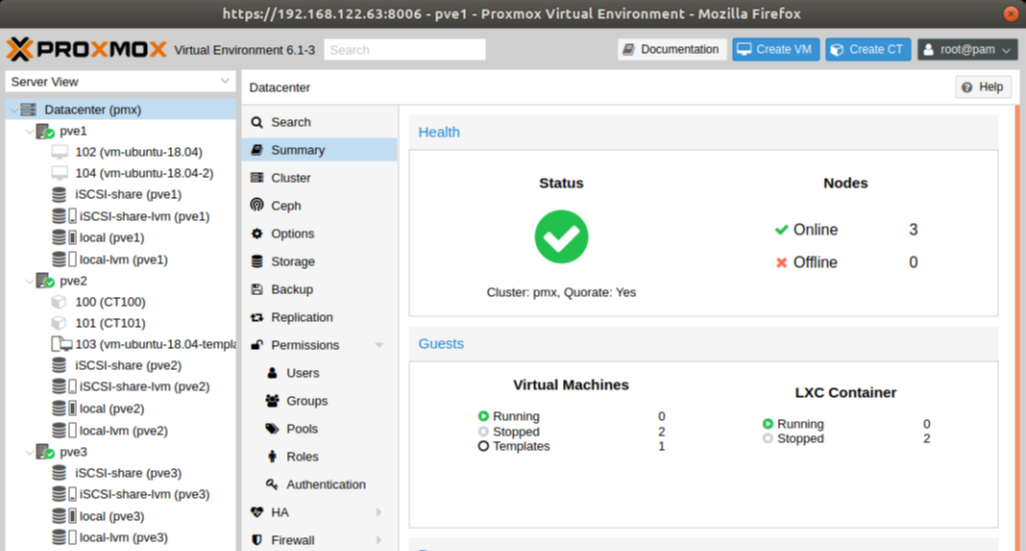
\includegraphics[width=1\textwidth]{9.png}}\\ 
    \href{https://developer.ibm.com/articles/l-virtio/}{\small\textit{Высокоуровневая архитектура фреймворка Virtio}} 
    \label{framework} 
\end{figure}

\begin{figure}[h]
    \centering
    \scalebox{0.9}{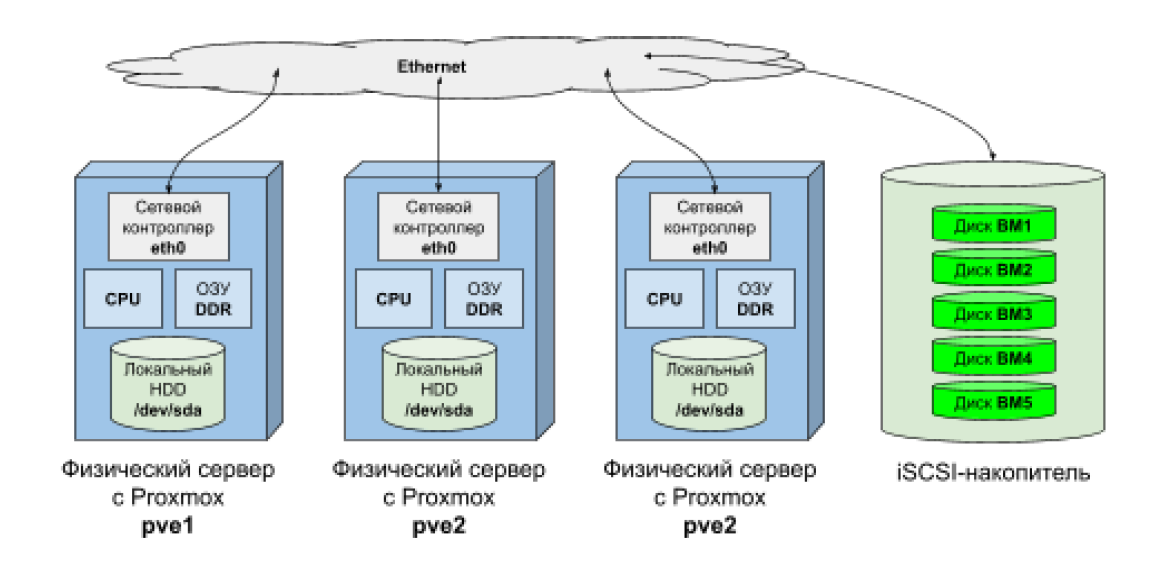
\includegraphics[width=1\textwidth]{10.png}}\\ 
    \small\textit{Архитектура VirtIO,}\href{https://projectacrn.github.io/latest/developer-guides/hld/hld-virtio-devices.html#architecture}{\small\textit{документация Project ACRN}} 
    \label{framework} 
\end{figure}

Высокая эффективность VirtIO достигается во многом благодаря механизму обмена данными между
хозяйской и гостевыми системами — Virtqueue. Две системы обмениваются данными через набор
буферов в разделяемой или общей памяти. Имеется в виду область памяти, доступная одновременно
обеим системам. То есть не нужно эмулировать десятки регистров управления и индивидуальных
битов в них. Эта же особенность позволяет существенно упростить драйверы, используемые в
гостевой системе. Также доступ к общей памяти не приводит к возникновению дополнительных
накладных расходов.\\

Дополнительные преимущества VirtIO состоят в том, что на стороне хозяйской системы может
использоваться любое устройство, поддерживаемое хозяйской системой. Более того, вместо
реального устройства можно использовать файл. Например, вместо реального накопителя с данными
может быть использован файл на местной или даже удалённой файловой системе.\\

Стоит заметить, что VirtIO-устройства используются не только в гостевых системах на основе ядра
Linux, но и в Microsoft Windows. Всё, что нужно для использования в Windows VirtIO устройств —
установить \href{http://www.linux-kvm.org/page/WindowsGuestDrivers}{соответствующие драйверы}, доступные для свободной загрузки. Однако у драйверов для
VirtIO есть одна неприятная особенность: доступные для свободного скачивания драйверы не имеют
WHQL-подписи Microsoft, которая есть у драйверов, являющихся частью Red Hat Enterprise Linux. Это
стоит иметь в виду, так как драйверы без WHQL-подписи имеют некоторые особенности при установке
и использовании.\\

\href{https://ru.wikipedia.org/wiki/WHQL}{\textbf{WHQL}} (сокр. от англ. Windows Hardware Quality Lab) — обозначение специальной лаборатории
фирмы Microsoft, занимающейся проверкой совместимости оборудования с операционными
системами Windows.\\

Microsoft Windows 10, начиная с версии 1607 Anniversary update, \href{https://techcommunity.microsoft.com/t5/Windows-Hardware-Certification/Driver-Signing-changes-in-Windows-10-version-1607/ba-p/364894}{более не загружает драйверы,
являющиеся модулями ядра}, если они не имеют WHQL-подписи Microsoft.

\subsubsection*{Microsoft Hyper-V Virtual Machine Bus} 
\addcontentsline{toc}{subsubsection}{Microsoft Hyper-V Virtual Machine Bus}

Если теперь, после рассмотрения фреймворка Virtio, взглянуть на Microsoft Hyper-V, внимательный
читатель наверняка обнаружит сходства в устройстве механизма паравиртуализации, который
используется для так называемых enlightened (по-русски — «просвещённых») гостевых систем.\\

Высокоуровневая архитектура гипервизора Hyper-V состоит из следующих компонентов:

\begin{enumerate}
    \item \textbf{VSC} (Virtualization Service Provider) — по сути, драйвер виртуального устройства в гостевой
    системе («дочернем разделе» в терминологии Microsoft Hyper-V).
    \item \textbf{VMBus} — интерфейс взаимодействия нескольких разделов. В основном, естественно,
    дочернего раздела (то есть гостевой системы) и корневого раздела, содержащего ОС Windows
    10 или Windows Server, которая работает в паре с гипервизором и обслуживает гостевые
    системы.
    \item \textbf{bVSP} (Virtualization Service Provider) — ответная часть виртуального устройства,
    предоставляющая требуемые сервисы клиенту в виртуальной машине.
\end{enumerate}

\begin{figure}[h]
    \centering
    \scalebox{1}{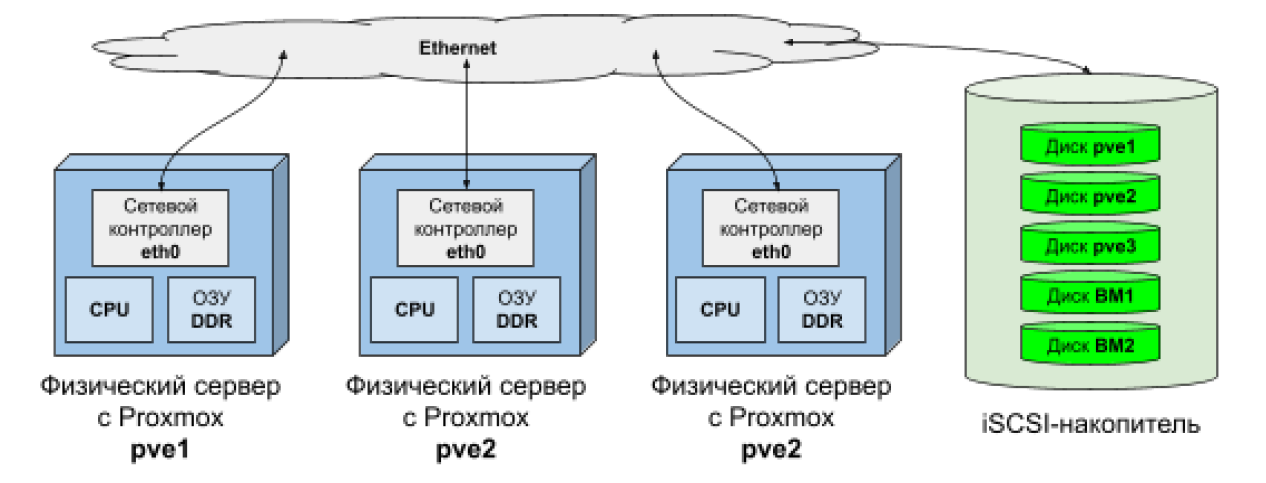
\includegraphics[width=1\textwidth]{11.png}}\\ 
    \href{https://docs.microsoft.com/ru-ru/virtualization/hyper-v-on-windows/reference/hyper-v-architecture}{\small\textit{Архитектура Microsoft Hyper-V}} 
    \label{framework} 
\end{figure}

Как и в случае с VirtIO, соответствующие паравиртуализованные устройства могут быть использованы
не только в «родных» ОС Microsoft Windows, но также в некоторых Linux-дистрибутивах и 
\href{https://docs.microsoft.com/ru-ru/windows-server/virtualization/hyper-v/supported-linux-and-freebsd-virtual-machines-for-hyper-v-on-windows}{ОС FreeBSD}. 
И точно так же, как VirtIO, VMBus позволяет существенно оптимизировать работу гостевых
систем с устройствами ввода-вывода, то есть в конечном счёте повысить эффективность системы
виртуализации.

\section*{Проброс оборудования} 
\addcontentsline{toc}{section}{Проброс оборудования}

Мы поговорили об эмуляции оборудования, которая привносит существенные накладные расходы, но
даёт полную свободу в выборе оборудования, позволяя использовать имеющиеся в гостевой системе
драйверы. И о паравиртуализации, которая требует реализации специфических виртуальных
устройств в гипервизоре и наличия соответствующих драйверов в гостевой системе, но зато
накладные расходы на работу паравиртуализованных устройств могут быть существенно сокращены.\\

Однако есть ещё один метод работы с оборудованием из гостевых систем — проброс оборудования в
гостевую систему. В английском варианте — passthrough, что дословно означает «проходить
насквозь».\\

В случае проброса оборудования гостевая система использует его напрямую, почти без
вмешательства гипервизора. Это позволяет достичь эффективности, близкой к реальной системе без
виртуализации, и реализовать максимальную скорость работы.

\begin{figure}[h]
    \centering
    \scalebox{0.9}{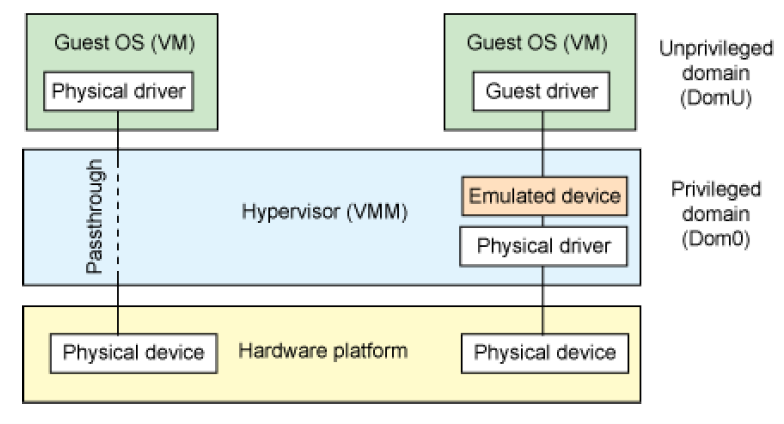
\includegraphics[width=1\textwidth]{12.png}}\\ 
    \small\textit{Проброс сквозь гипервизор,} \href{https://developer.ibm.com/tutorials/l-pci-passthrough/}{\small\textit{Linux virtualization and PCI passthrough}} 
    \label{framework} 
\end{figure}

Проброс оборудования в гостевую систему имеет смысл делать не только для достижения
экстремальной производительности. Он применим и в случае использования устройств, которые по
своей природе сложно или невозможно разделить между несколькими гостевыми системами или хотя
бы между гипервизором и одной из гостевых систем. За примерами ходить далеко не надо:
последовательный порт, USB-устройства, графические процессоры (GPU).\\

Проброс оборудования был бы невозможен без важной инновации от производителей процессоров.
Эта инновация, обычно называемая просто IOMMU, была разработана и представлена компаниями
Intel (под названием Virtualization Technology for Directed I/O или сокращённо VT-d) и AMD (под
названием I/O Memory Management Unit или сокращённо, собственно, IOMMU) почти одновременно в
2010–2011 годах.\\

Аппаратура IOMMU, предварительно настроенная гипервизором, позволяет гостевым системам
работать с памятью внешних устройств, а также прерываниями, поступающими от этих устройств, так,
как если бы гостевые системы, работали с аппаратурой, будучи хозяйской системой, запущенной на
данной аппаратуре. При этом IOMMU незаметно (или, как ещё говорят, «прозрачно») для гипервизора
и гостевой системы выполняет трансляцию адресов, используемых гостевой системой, в физические
адреса, используемые аппаратурой, и наоборот. А также перенаправляет прерывания к обработчикам
прерываний гостевой системы. При попытках гостевой системы получить доступ к ресурсам, таким как
память и прерывания, которые не были зарегистрированы гипервизором как доступные данному
гостю, IOMMU генерирует исключительную ситуацию, которую в штатном режиме обрабатывает
гипервизор.\\

Надеемся, теперь понятна оговорка, сделанная выше, что в случае проброса оборудования гостевая
система работает с оборудованием почти без участия гипервизора.\\

Но есть у проброса оборудования и существенный недостаток, особенно важный в системах
серверной виртуализации. Это сложность обеспечения миграции гостевых систем, использующих
проброс оборудования. Как мы узнали из предыдущих глав, миграция виртуальной машины с одного
физического сервера на другой — это давно решённая задача. Гипервизор создаёт некое
универсальное окружение для гостевой системы, и это окружение можно реализовать даже на
серверах, имеющих весьма отличную конфигурацию: модель центрального процессора, размер и
размещение накопителя данных, набор устройств ввода-вывода и т. д. Привязка гостевой системы к
конкретному экземпляру аппаратуры существенно усложняет миграцию такого гостя. Как минимум
миграция должна происходить на машину, обладающую таким же устройством. Более того, необходим
механизм, позволяющий на лету приостанавливать и затем возобновлять работу проброшенного
устройства.\\

В теории шины PCI и PCI Express поддерживают так называемое горячее подключение, или hot-plug.
Но сама по себе возможность на лету подключать и отключать устройства не решает вопрос
неожиданного прерывания работы и её возобновления на другой аппаратуре. Нужно перенести с
одной машины на другую данные, оставшиеся во внутренней памяти ранее использованного
устройства, и его внутренние состояния.

\section*{Драйверы в пространстве пользователя} 
\addcontentsline{toc}{section}{Драйверы в пространстве пользователя}

И снова мы, казалось бы, рассмотрели все возможные варианты обеспечения высокой
эффективности совместно с высокой производительностью. Но нет, есть ещё одна набирающая
популярность технология — драйверы в пространстве пользователя. Сама по себе концепция не
связана непосредственно с виртуализацией. Идея состоит в том, чтобы исключить ядро ОС из
взаимодействия ПО, осуществляющего какую-то полезную работу с данными, и, собственно,
аппаратуры, предоставляющей эти данные.\\

В случае обычного взаимодействия ПО и аппаратуры обработка данных фактически происходит
дважды: ядро ОС получает данные непосредственно из аппаратуры и помещает их в буфер,
предоставленный ПО пользователя, и только затем пользовательское ПО совершает какую-то
полезную работу над этими данными. Точно так же в обратную сторону. В таком процессе
невооружённым глазом видны как минимум две неприятные особенности:

\begin{enumerate}
    \item \textbf{Дополнительное копирование данных из буфера, используемого устройством, в буфер,
    используемый ПО пользователя}. И так же в обратную сторону. Очевидно, что копирование
    данных, ещё и в большом объёме, негативно сказывается на производительности системы,
    так как приводит к «вымыванию» кешей процессора, возникновению дополнительных отказов
    страниц и банальной загрузке шины данных.

\noindent   \href{https://ru.wikipedia.org/wiki/Отказ_страницы}{\textbf{Отказ страницы}} (англ. Page fault) — разновидность аппаратного исключения, возникающего в
\noindent компьютере с виртуальной памятью на основе подкачки страниц в момент обращения к странице 
памяти, которая не включена блоком управления памятью в виртуальное адресное пространство
процесса.
\item \textbf{Многократные переключения из контекста пользовательского процесса в контекст ядра
и обратно}. Из-за использования разных адресных пространств, как и в случае
дополнительного копирования данных, вымываются кеши данных и MMU (имеется в виду
содержимое TLB).
\end{enumerate}

\href{https://ru.wikipedia.org/wiki/Буфер_ассоциативной_трансляции}{\textbf{Буфер ассоциативной трансляции}} (англ. Translation lookaside buffer, TLB) — это специализированный
кеш центрального процессора, используемый для ускорения трансляции адреса виртуальной памяти
в адрес физической памяти.\\

Пользовательскому приложению можно дать доступ ко всем управляющим регистрам аппаратуры, а
также подготовить буферы ввода-вывода таким образом, чтобы они были заранее доступны в
адресном пространстве пользовательского приложения. Более того, поскольку обработка прерываний
возможна только из максимально привилегированного режима, то есть либо из хозяйской ОС, либо из
гипервизора, мы откажемся от использования прерываний. Вместо этого приложение пользователя
будет работать в так называемом \href{https://en.wikipedia.org/wiki/Polling_(computer_science)}{режиме опроса}. То есть вместо ожидания аппаратного сигнала
процессору, по которому будет выполнен обработчик этого события (прерывания), приложение
пользователя само периодически вычитывает значение из регистра состояния аппаратуры. Если оно
обнаруживает флаг, сигнализирующий о наступлении определённого события, приложение выполняет
необходимые действия.\\

Это может показаться удивительным, но применительно к высокопроизводительным устройствам
ввода-вывода использование прерываний оказывается гораздо менее эффективным, чем
периодический опрос регистров состояния из ПО, будь то пользовательское ПО или драйвер самой
ОС. Дело в том, что обычно аппаратура генерирует прерывание на каждое элементарное событие.\\

Например, сетевой контроллер может генерировать прерывание в случае отправки и получения
каждого \href{https://ru.wikipedia.org/wiki/Maximum_transmission_unit}{пакета с данными}, размер которого обычно около 1,5 килобайт. При использовании самой
обыкновенной сети 1Gb Ethernet со скоростью передачи данных 1 гигабит/сек., 1 500 байт (или 1 500 *
8 = 12 000 бит) будут переданы за 12 микросекунд. Современный процессор, работающий на частоте
2,5 ГГц, может выполнять порядка 2,5 миллиардов команд в секунду. Таким образом, за время,
требующееся на передачу 1,5 килобайт данных, современный процессор выполнит лишь около 30 000
команд.\\

В реальности на обработку прерывания от сетевого контроллера с учётом затрат на переключение
контекста из режима пользователя в режим ядра и прочее может запросто уйти соизмеримое
количество команд процессора. Другими словами, даже современный процессор может оказаться
занят почти полностью только получением и отправкой пакетов по сети. Это вряд ли похоже на
эффективное использование аппаратуры. Также стоит помнить, что современные сети в центрах
обработки данных, как правило, имеют скорость работы 2,5 или даже 10 гигабит/сек. При этом,
разумеется, времени на обработку прерываний оставалось бы ещё меньше. Выходом становится
обработка сразу набора пакетов время от времени. При этом существенно снижаются накладные
расходы на переключение контекста.\\


\begin{figure}[h]
    \centering
    \scalebox{0.9}{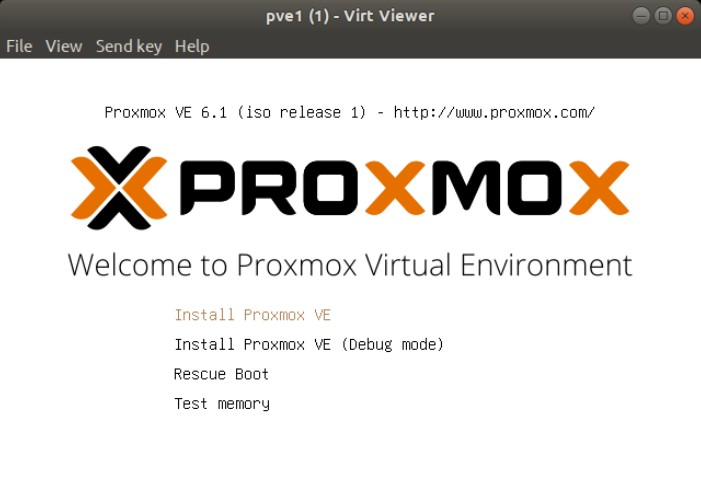
\includegraphics[width=1\textwidth]{13.png}}\\  
    \label{framework} 
\end{figure}

\subsection*{DPDK} 
\addcontentsline{toc}{subsection}{DPDK}

\begin{figure}[h]
    \centering
    \scalebox{0.5}{
\includegraphics[width=1\textwidth]{14.png}}\\ 
    \small\textit{\href{http://fast.dpdk.org/download/logos/}{DPDK Logo} under CC BY-ND 4.0 license}  
    \label{framework} 
\end{figure}

Одно из наиболее известных и популярных на сегодняшний день применений описанного выше
подхода — проект \href{https://www.dpdk.org/}{Data Plane Development Kit} (DPDK). В рамках проекта DPDK разрабатываются:

\begin{itemize}
    \item драйверы для сетевых контроллеров: как для реальной аппаратуры, так и для виртуальных
    интерфейсов популярных гипервизоров, таких как VMware ESXi, Microsoft Hyper-V, Xen и KVM;
    \item драйверы для операционных систем Linux, Windows и FreeBSD;
    \item набор библиотек для использования в конечных приложениях, которые при использовании на
    поддерживаемой аппаратуре позволяют существенно ускорить работу сетевых приложений.
\end{itemize}

Интересно, что этот проект развивается под эгидой Linux Foundation и все компоненты, включая
исходный код библиотек и драйверов, а также документация доступны для изучения всем желающим.\\

\begin{figure}[h]
    \centering
    \scalebox{0.8}{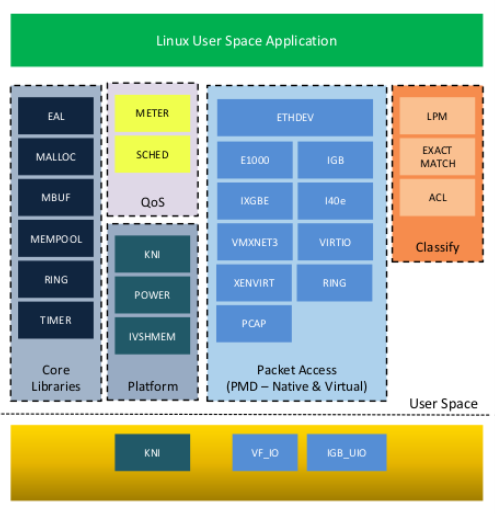
\includegraphics[width=1\textwidth]{15.png}}\\ 
    \small\textit{Высокоуровневая архитектура DPDK,\\
    \href{https://www.slideshare.net/jstleger/dpdk-summit-2015-intel-keith-wiles}{Future enhancements to DPDK framework}, DPDK Summit 2015, Keith Wiles, Intel}  
    \label{framework} 
\end{figure}

В настоящее время DPDK стал стандартом де-факто для высокопроизводительных сетевых
приложений. Именно на DPDK ориентируются производители мощных сетевых контроллеров для
центров обработки данных, а также поставщики облачной инфраструктуры, хостинг-провайдеры и т. д.
Так что стоит обратить на DPDK внимание, благо в свободном доступе есть официальная
документация, а также множество статей, записей выступлений и т. д.

\section*{Сетевая инфраструктура} 
\addcontentsline{toc}{section}{Сетевая инфраструктура}

Поскольку в данном курсе мы в основном говорим о серверной виртуализации, то вопросы обмена
данными по сети между виртуальными машинами и другими устройствами в локальной и глобальной
сетях — важный для нас аспект функционирования систем виртуализации. Скорее всего, сетевой
интерфейс — это единственное средство взаимодействия виртуальной машины со внешним миром.\\

Сетевой инфраструктуре в случае использования виртуальных машин нужно маршрутизировать
пакеты с данными из внешней сети до конкретной виртуальной машины и в обратную сторону. В
случае физических машин, серверов с реальными сетевыми адаптерами, имеющими подключение к
сети, задача маршрутизации пакетов возложена на специализированную аппаратуру:
маршрутизаторы и коммутаторы.\\

\href{https://ru.wikipedia.org/wiki/Маршрутизатор}{\textbf{Маршрутизатор}} (проф. жарг. рýтер или роутер, транслитерация от англ. router) —
специализированный компьютер, который пересылает пакеты между различными сегментами сети на
основе правил и таблиц маршрутизации.\\

\href{https://ru.wikipedia.org/wiki/Сетевой_коммутатор}{\textbf{Сетевой коммутатор}} (жарг. свитч, свич, от англ. switch — «переключатель») — устройство,
предназначенное для соединения нескольких узлов компьютерной сети в пределах одного или
нескольких сегментов сети.\\

В случае выделения каждой виртуальной машине своего реального сетевого адаптера можно точно
так же полагаться на внешнюю маршрутизацию. Однако описанный ранее вариант использования
сетевых адаптеров достаточно редко встречается на практике. Хотя бы потому, что пропускной
способности одного или нескольких сетевых адаптеров сервера может быть более чем достаточно на
все запущенные (а их могут быть десятки) виртуальные машины. В таком случае встаёт вопрос
маршрутизации пакетов в рамках одного физического сервера между виртуальными машинами,
запущенными на нём.\\

Самое простое решение для маршрутизации пакетов между гостевыми системами и внешним миром
могло бы состоять в создании для каждой виртуальной машины своего логического сетевого
интерфейса и добавлении его в сетевой мост вместе с реальным сетевым адаптером хозяйской
системы.\\

\href{https://ru.wikipedia.org/wiki/Сетевой_мост}{\textbf{Сетевой мост}} (также «бридж» от англ. bridge) — сетевое устройство второго уровня модели OSI,
предназначенное для объединения сегментов (подсети) компьютерной сети в единую сеть.\\

Красота этого решения состоит в том, что современные ОС и гипервизоры имеют встроенную
поддержку программных сетевых мостов. То есть, казалось бы, проблема решена. Но у сетевого
моста есть ряд недостатков, которые становятся весьма существенными, когда речь идёт о системе
виртуализации.\\

Во-первых, реализация сетевого моста подразумевает простую пересылку данных из одного сетевого
интерфейса, входящего в мост, во все остальные. То есть все сетевые интерфейсы, входящие в
данный мост, будут получать данные из внешнего мира, адресованные любому из участников моста, а
также данные от всех прочих участников моста, адресованные внешнему миру. Тут возникает как
минимум несколько проблем:

\begin{enumerate}
    \item Все сетевые интерфейсы, входящие в данный мост, вынуждены обрабатывать пакеты с
    данными, которые им совершенно не нужны. Это создает излишнюю и бессмысленную
    нагрузку на центральный процессор каждой системы.\\

    Хуже того, поскольку канонический мост предназначен, чтобы связать, как обычный кабель, несколько
сегментов сети, в общем случае не зная, какие системы находятся по разные стороны моста,
ретрансляции подвергаются все до единого пакеты, путешествующие по любому из подключённых
сегментов сети. Для этого сетевой адаптер хозяйской машины переводится в так называемый
«неразборчивый» режим (англ. promiscuous mode). В нормальном же режиме работы сетевой
адаптер автоматически отбрасывает все пакеты, кроме тех, что адресованы конкретно ему. Выбор
происходит по MAC-адресу узла назначения. Таким образом, в нормальном режиме работы
центральный процессор хозяйской системы затрачивает свои вычислительные ресурсы только на
обработку пакетов, адресованных конкретно ему. В «неразборчивом» же режиме ЦП хозяйской
системы вынужден заниматься обработкой каждого пакета, путешествующего по сети. Можно себе
только представить, какие накладные расходы возникают при использовании сервера в
высоконагруженной 10-гигабитной сети!
\item Сетевые интерфейсы пропускают через себя и свои данные, и данные, адресованные другим
системам. В таком случае значительно осложняется задача корректного подсчета объёма
переданных и принятых данных.
\item Поскольку все интерфейсы получают данные, адресованные всем, могут возникать
неприятные ситуации с получением доступа к данным, которые не хотелось бы делать
доступными случайным получателям. Не стоит рассчитывать на полноценную изоляцию
передаваемых по сети данных. Если требуется надёжный обмен конфиденциальными
данными, стоит использовать шифрование данных вместо наивных попыток правильно эти
данные адресовать. Стоит отдавать себе отчёт, что даже VLAN (Virtual Local Area Network,
виртуальная локальная сеть) не делает обмен данными хоть сколько-то безопасным, так как
фактически данные передаются через ту же аппаратуру, что и у других VLAN. Она лишь
несколько упрощает администрирование сети.
\end{enumerate}

Кроме того, мы же помним, что одна из ключевых особенностей современных систем виртуализации
— возможность динамически управлять виртуальными машинами: создавать и уничтожать
виртуальные машины по мере необходимости, а также переносить работающие виртуальные машины
с одного физического сервера на другой. Причём миграция виртуальной машины приводит к
изменению не только заранее заданной конфигурации сети (выданных адресов и жёстко заданных
маршрутов), но также и состояния сети, сформированного в реальном времени (таблиц динамической
трансляции адресов и тому подобного). И вот тут уже не поможет никакой сетевой мост.\\

Нужно что-то другое — более гибкое и мощное средство маршрутизации, способное динамически
менять правила маршрутизации, тесно взаимодействуя с работающими гипервизорами или
системами управления гипервизорами. Ниже мы рассмотрим несколько популярных продуктов,
решающих эти задачи.

\subsection*{VMware ESXi vSwitch} 
\addcontentsline{toc}{subsection}{VMware ESXi vSwitch}

Начнём свой обзор конкретных решений с предложений компании VMware, которая, как мы помним,
была и остаётся пионером и лидером на рынке современной серверной виртуализации. Запуск
нескольких, а то и множества виртуальных машин на одном сервере — это типичная ситуация. Можно
даже сказать, что обратная ситуация с запуском лишь одной ВМ на сервере весьма нетипична.
Соответственно, гипервизору необходимо заниматься маршрутизацией пакетов с данными между
реальным сетевым адаптером (NIC — Network Interface Controller) и виртуальными сетевыми
адаптерами (vNIC — Virtual NIC).\\

Разумеется, монолитный гипервизор ESXi компании VMware способен справиться и с такой задачей.
Для этого в составе ESXi предусмотрен виртуальный L2-коммутатор, имеющий незамысловатое
название vSphere Switch. На самом деле vSwitch существует в двух вариантах. Изначально
использовался vSphere Standard Switch, занимающийся маршрутизацией между виртуальными
машинами под управлением одного гипервизора, то есть в рамках одной хозяйской машины.

\begin{figure}[h]
    \centering
    \scalebox{0.8}{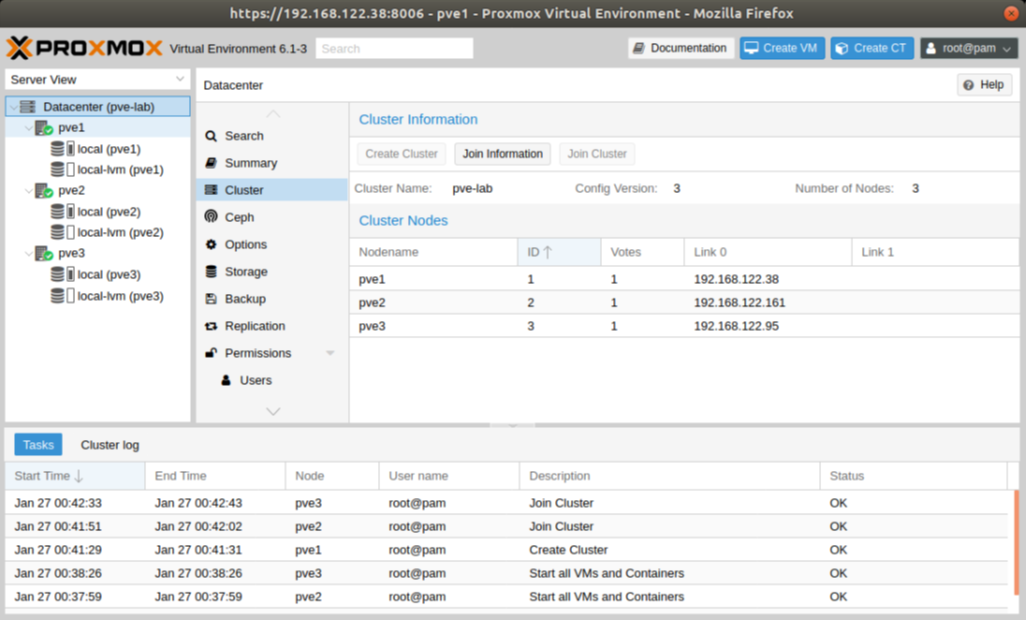
\includegraphics[width=1\textwidth]{16.png}}\\ 
    \small\textit{Сеть с использованием vSphere Standard Switch, \href{https://docs.vmware.com/en/VMware-vSphere/index.html}{документация на vSphere 5}}  
    \label{framework} 
\end{figure}

А с выходом vSphere 4.0 появился vSphere Distributed vSwitch, который занимается управлением
виртуальной сетевой инфраструктурой при использовании нескольких серверов и гипервизоров.

\newpage

\begin{figure}[h]
    \centering
    \scalebox{0.8}{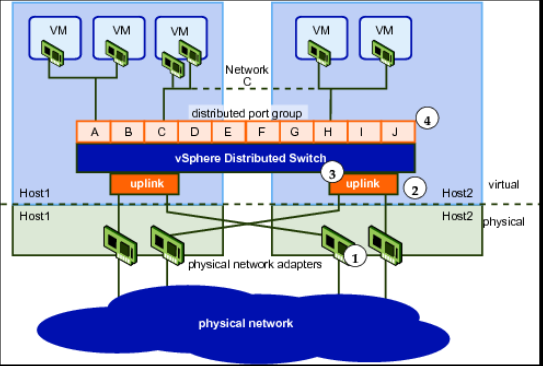
\includegraphics[width=1\textwidth]{17.png}} \\
    \small\textit{Сеть с использованием vSphere Distributed Switch, \href{https://docs.vmware.com/en/VMware-vSphere/index.html}{документация на vSphere 5}} 
    \label{framework} 
\end{figure}

\textbf{vSphere Switch решает следующие задачи:}
    \begin{enumerate}
        \item Обеспечение безопасности: доступ по MAC-адресу, управление «неразборчивым» режимом.
        \item Управление шейпингом передаваемых данных: задание средней и максимальной полосы
        пропускания и т. д. Применимо только к исходящим данным.
        \item Управление совместной работой сетевых интерфейсов.
        \item Управление балансировкой нагрузки с учётом конкретных виртуальных сетевых интерфейсов,
        MAC-адресов и прочих политик.
        \item Обеспечение работы виртуальных подсетей (VLAN, IEEE 802.1Q).
    \end{enumerate}

\href{https://ru.wikipedia.org/wiki/Шейпинг_(информатика)}{\textbf{Шейпинг}} (англ. shaping traffic — придание трафику формы) — ограничение пропускной способности
канала для отдельного узла сети ниже технических возможностей канала до узла. Шейпинг обычно
используется как средство ограничения максимального потребления трафика со стороны узла сети.\\

В добавление к этим задачам \href{https://kb.vmware.com/s/article/1010555}{vSphere Distributed Switch предлагает}:
\begin{enumerate}
    \item Зеркалирование потока данных при помощи стандартных протоколов SPAN (Switched Port
    Analyzer), RSPAN (Remote Switched Port Analyzer) и ERSPAN (Encapsulated Remote Switch Port
    Analyzer).
    \item Мониторинг данных при помощи NetFlow.
    \item Шейпинг входящих данных.
    \item Централизованное управление конфигурацией через интерфейс vCenter Server.
\end{enumerate}

Стоит, однако, заметить, что в отличие от vSphere Standard Switch, являющегося частью собственно
гипервизора, и, соответственно, доступного даже при использовании VMware ESXi в бесплатном
режиме (для личных нужд, например), распределённый сетевой коммутатор vSphere Distributed Switch
доступен только как часть продукта vSphere в версии Enterprise Plus и более высоких (читай: дорогих).

\subsection*{Open vSwitch} 
\addcontentsline{toc}{subsection}{Open vSwitch}

Следующим решением, на которое мы обратим внимание, будет Open v- Switch — очень популярный
виртуальный многоуровневый коммутатор с открытым исходным кодом. Open vSwitch был разработан
небольшой командой инженеров из компании Nicira. Компания Nicira основана Мартином Касадо
(Martin Casado), Ником МакКоун (Nick McKeown) и Скоттом Шенкером (Scott Shenker) в 2007 году. В
июле 2012 года \href{https://news.vmware.com/releases/vmware-to-acquire-nicira}{была приобретена компанией VMware}.\\

Будучи проектом с открытым исходным кодом, Open vSwitch — часто можно встретить сокращение
OVS — продолжил своё существование и снискал ещё большую популярность благодаря доступности
(он абсолютно бесплатен), высокой функциональности и гибкости конфигурирования. А в августе 2016
года Open vSwitch перешёл под покровительство Linux Foundation.
В настоящее время Open vSwitch используется как коммутатор по умолчанию для Xen Open Cloud
Platform, но также может интегрироваться с разнообразными гипервизорами, такими как Xen, KVM,
Oracle VirtualBox и даже Microsoft Hyper-V.\\

Что интересно, в марте 2017 года компания VMware \href{https://blogs.vmware.com/networkvirtualization/2017/03/native-vswitch.html/}{заявила о прекращении поддержки сторонних
виртуальных коммутаторов}, желая сфокусироваться всего на двух решениях: vSphere Standard и
Distributed Switch для VMware vSphere и Open vSwitch. Тем не менее до сих пор в Open vSwitch
отсутствует интеграция с гипервизорами VMware.\\

Хотя Open vSwitch стартовал как сугубо программный продукт, предназначенный изначально для
запуска на системах под управлением ядра ОС Linux, сейчас ведётся активная работа по
портированию Open vSwitch на реальные сетевые системы на кристалле (SoC), а также ускорению
работы Open vSwitch благодаря \href{https://www.netronome.com/m/documents/WP_Netronome_25GbE_SmartNICs_with_Open_vSwitch_Hardware_Offload.pdf}{перемещению ряда задач на соответствующие сетевые контроллеры}
или их части. Open vSwitch, как правило, представляет собой модуль ядра Linux, но также может
работать и в пространстве пользователя как обычное приложение, однако, разумеется, не так
эффективно, как в пространстве ядра.\\

\begin{figure}[h]
    \centering
    \scalebox{0.8}{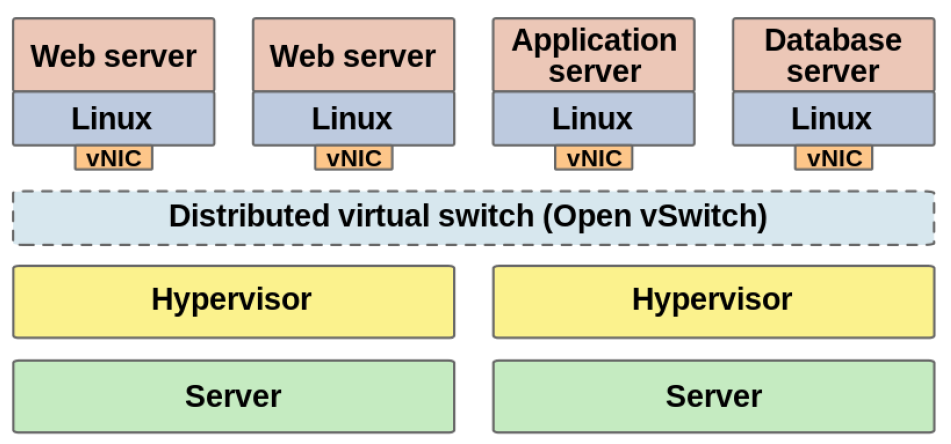
\includegraphics[width=1\textwidth]{18.png}} \\
    \small\textit{\href{https://commons.wikimedia.org/wiki/File:Distributed_Open_vSwitch_instance.svg}{Distributed Open vSwitch instance}, \href{https://commons.wikimedia.org/wiki/User:Goran_tek-en}{Goran tek-en} на условиях лицензии CC BY-SA 4.0} 
    \label{framework} 
\end{figure}

Благодаря развитым программным интерфейсам и встроенным возможностям по интеграции с
широко используемыми гипервизорами (за исключением разве что VMware ESXi), Open vSwitch
позволяет автоматизировать управление сетью, состоящей из множества виртуальных машин.\\

\textbf{Другие важные особенности Open vSwitch:}
\begin{itemize}
    \item Поддержка таких стандартных протоколов, как NetFlow, sFlow, Switched Port Analyzer
    (SPAN)/Remote Switched Port Analyzer (RSPAN), LACP и 802.1ag.
    \item Поддержка VLAN (IEEE 802.1Q).
    \item Поддержка механизма QoS для различных приложений, пользователей или даже потоков
    обработки данных.
    \item Возможность агрегации портов с распределением нагрузки благодаря протоколу Link
    Aggregation Control Protocol (LACP, IEEE 802.1AX-2008).
    \item Поддержка множества протоколов туннелирования, включая GRE, Virtual Extensible LAN
    (VXLAN), Stateless Transport Tunneling (STT) и IPSec.
    \item Совместимость с программным мостом Linux Bridge (brctl).
\end{itemize}

\href{https://ru.wikipedia.org/wiki/QoS}{\textbf{QoS}} (англ. quality of service — «качество обслуживания») — технология предоставления различным
классам трафика различных приоритетов в обслуживании. Также этим термином в области
компьютерных сетей называют вероятность того, что сеть связи соответствует заданному соглашению
о трафике. В ряде случаев — неформальное обозначение вероятности прохождения пакета между
двумя точками сети.\\

Как мы видим, Open vSwitch — функциональный аналог VMware vSphere Distributed Switch. Он
реализует даже более широкий спектр возможностей, оставаясь совершенно бесплатным.\\

Ознакомиться более подробно с возможностями Open vSwitch можно в статье на английской
«Википедии» или в официальной документации на сайте проекта. Статья на русском на сегодняшний
день лишь даёт определение, не более того.

\subsection*{Microsoft Hyper-V Virtual Switch} 
\addcontentsline{toc}{subsection}{Microsoft Hyper-V Virtual Switch}

Как и в случае проприетарного гипервизора компании VMware со встроенным виртуальным
коммутатором, решение для виртуализации от компании Microsoft имеет собственный виртуальный
коммутатор второго уровня, называемый, соответственно, Hyper-V Virtual Switch. Как и ранее
рассмотренные виртуальные коммутаторы, Hyper-V Virtual Switch служит для связи виртуальных
сетевых интерфейсов и виртуальных машин с реальной внешней сетью, обеспечивая примерно тот
же набор базового функционала: сбор и отображение статистики событий в сети, шейпинг данных,
зеркалирование портов и т. д.\\

Однако есть и несколько существенных отличий от ранее рассмотренных решений.\\

Во-первых, Hyper-V Virtual Switch работает исключительно в рамках одного Hyper-V гипервизора, то
есть одного физического сервера. Во всяком случае, на момент написания данного материала, то
есть в конце 2019 года. При миграции виртуальной машины с одной хозяйской системы на другую
гипервизор, владеющий в данный момент виртуальной машиной, попытается обнаружить
виртуальный коммутатор с точно таким же названием на целевом гипервизоре, куда
предположительно будет осуществлена миграция. Если коммутатор с таким же именем не будет
найден, то миграции не произойдёт. Возможно, в будущем компания Microsoft расширит функционал
своего виртуального коммутатора, но пока он скорее похож на стандартный коммутатор из состава
гипервизора ESXi, чем на vSphere Distributed Switch или Open vSwitch.\\

Второе важное отличие (в основном от виртуального коммутатора \\ VMware) состоит в возможности
создавать \href{https://learn.microsoft.com/en-us/windows-hardware/drivers/network/hyper-v-extensible-switch-extensions}{свои расширения для виртуального коммутатора}. И именно благодаря этой возможности
удалось реализовать интеграцию гипервизора Hyper-V c Open vSwitch. Более подробную информацию
о том, как эта интеграция реализована, можно найти в \href{https://docs.openvswitch.org/en/latest/topics/windows/}{документации на Open vSwitch}.\\

Еще одно интересное отличие от ранее рассмотренных коммутаторов — три выделенных режима
работы: Private (частный), Internal (внутренний) и External (внешний) virtual switch.

\begin{enumerate}
    \item В режиме Private virtual switch сетевые интерфейсы виртуальных машин, подключённых к
    коммутатору, могут обмениваться данными только друг с другом, но не имеют возможности
    получить доступ даже к корневому разделу (англ. root partition — «административной ОС» в
    терминологии Hyper-V), не говоря уже о внешней сети. Такой режим может оказаться
    полезным, когда требуется строгая изоляция сети, к которой подключены гостевые системы.
    \item Режим Internal virtual switch добавляет возможность взаимного обмена данными гостевых и
    административной ОС.
    \item Режим External virtual switch добавляет подключение коммутатора к внешней сети через
    заданный реальный сетевой интерфейс или даже группу интерфейсов.
\end{enumerate}

Ниже наглядно проиллюстрированы все три режима:

\newpage

\begin{figure}[h]
    \centering
    \scalebox{1}{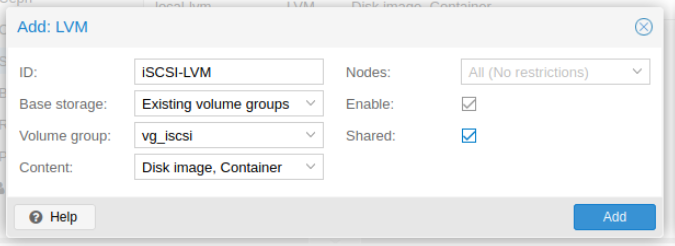
\includegraphics[width=0.44\textwidth]{19.png}} \\
    \label{framework} 
\end{figure}

\begin{figure}[h]
    \centering
    \scalebox{1}{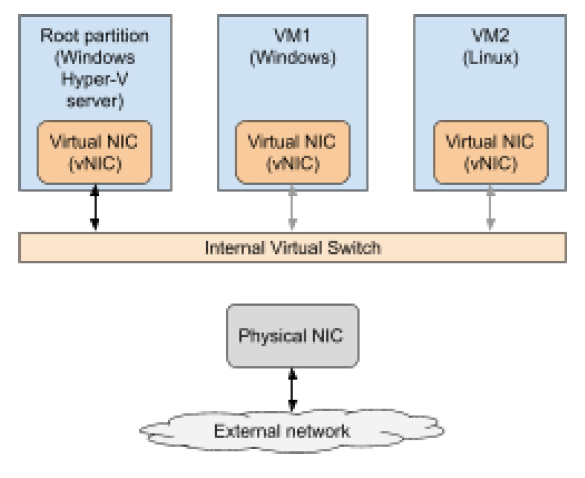
\includegraphics[width=0.44\textwidth]{20.png}} \\
    \label{framework} 
\end{figure}

\begin{figure}[h]
    \centering
    \scalebox{1}{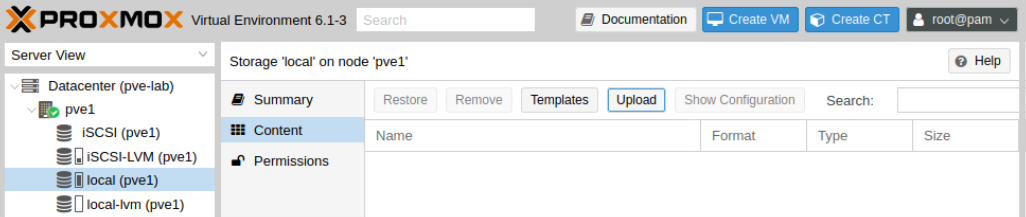
\includegraphics[width=0.44\textwidth]{21.png}} 
    \label{framework} 
\end{figure}

\newpage

\subsection*{Заключение} 
\addcontentsline{toc}{subsection}{Заключение}

Как мы увидели, рассмотрев несколько широко используемых виртуальных коммутаторов, они все
реализуют похожую базовую функциональность, но могут отличаться некоторыми деталями.
Проприетарные решения определённо тесно интегрированы с соответствующими гипервизорами, но
могут иметь некоторые особенности, такие как необходимость дополнительных инвестиций или
ограниченная функциональность. По сравнению с ними, открытый коммутатор Open vSwitch обладает
широчайшими возможностями, но могут быть сложности при интеграции с некоторыми
гипервизорами, например VMware ESXi. Тем не менее можно найти решение для настройки и
поддержания необходимой сетевой инфраструктуры любого современного гипервизора.\\

\section*{Используемые источники} 
\addcontentsline{toc}{section}{Используемые источники}

\begin{enumerate}
    \item \href{https://www.usenix.org/legacy/events/osdi10/tech/full_papers/Ben-Yehuda.pdf}{The Turtles Project: Design and Implementation of Nested Virtualization.}
    \item \href{https://www.linux-kvm.org/images/3/33/02x03-NestedVirtualization.pdf}{Nested Virtualization: State of the art and future directions}.
    \item \href{https://events19.linuxfoundation.org/wp-content/uploads/2017/12/Improving-KVM-x86-Nested-Virtualization-Liran-Alon-Oracle.pdf}{Improving KVM x86 nested virtualization}.
    \item \href{https://www.redhat.com/en/blog/inception-how-usable-are-nested-kvm-guests}{Inception: How usable are nested KVM guests}.
    \item \href{https://docs.microsoft.com/en-us/virtualization/hyper-v-on-windows/user-guide/nested-virtualization}{Run Hyper-V in a Virtual Machine with Nested Virtualization}.
    \item \href{https://www.kernel.org/doc/Documentation/virtual/kvm/timekeeping.txt}{Timekeeping Virtualization for X86-Based Architectures}.
    \item \href{https://www.kernel.org/doc/Documentation/virtual/kvm/timekeeping.txt}{Timekeeping in VMware Virtual Machines}.
    \item \href{https://developer.ibm.com/tutorials/l-pci-passthrough/}{Linux virtualization and PCI passthrough}.
    \item \href{https://it-events.com/system/attachments/files/000/001/102/original/LinuxPiter-DPDK-2015.pdf}{The Data Plane Development Kit (DPDK) – What it is and where it’s going}.
    \item \href{https://blog.selectel.ru/vvedenie-v-dpdk-arxitektura-i-princip-raboty/}{Введение в DPDK: архитектура и принцип работы}.
    \item \href{https://www.slideshare.net/jstleger/dpdk-summit-2015-intel-keith-wiles}{Future enhancements to DPDK framework}.
    \item \href{https://ivirt-it.ru/open-vswitch-cicle/}{Open vSwitch. Цикл статей}.
    \item \href{https://docs.vmware.com/en/VMware-vSphere/6.7/com.vmware.vsphere.networking.doc/GUID-35B40B0B-0C13-43B2-BC85-18C9C91BE2D4.html}{Документация на VMware vSphere Networking}.
    \item \href{https://www.altaro.com/hyper-v/the-hyper-v-virtual-switch-explained-part-1/}{What is the Hyper-V Virtual Switch and How Does it Work}.
    \item \href{http://www.itc22.com/fileadmin/ITC22_files/Edge_Talk-Pettit.pdf}{Virtual Switching in an Era of Advanced Edges}.
    \item \href{https://www.net.in.tum.de/fileadmin/bibtex/publications/papers/Open-vSwitch-CloudNet-14.pdf}{Performance Characteristics of Virtual Switching}.
\end{enumerate}

\section*{Практическое задание} 
\addcontentsline{toc}{section}{Практическое задание}

\begin{enumerate}
    \item Настройте вложенную виртуализацию на свой выбор: на хозяйской системе с
    Linux-дистрибутивом KVM или на хозяйской системе с Windows 10 Hyper-V.
    \item Оцените производительность гостевого гипервизора. Для простоты можно понаблюдать за
    отзывчивостью разных процессов, например, загрузкой и стартом различных приложений.
    Более точную оценку можно получить, воспользовавшись тестами из \href{https://www.phoronix-test-suite.com/}{Phoronix Test Suite}.
\end{enumerate}


\end{document}